\chapter{Concept}
\section{Tree Creation}
\label{sec:tree_creation_angle}
The ETH-Zurich already has genetic optimizations algorithms based on trees. Unfortunately they don't have a working solution to produce a tree from the existing graph. The new created tree generation algorithm produces a relative tree with absolute angles. This allowed an easier and faster work process with tree based structures.

To create a tree from an existing graph the angle and distance should be enough data to fully represent a graph.
Two approaches exist to define angles. One is to separate the circle range into minus and plus 180 degrees. This would allow to step straight forward with the angle 0 degree (Figure \ref{fig:tree-generation-decision} left). Another approach is to use the range from 0 to 360 degrees. In this case straight forward would be 180 degrees (Figure \ref{fig:tree-generation-decision} right).

\begin{figure}[!ht]
    \centering
    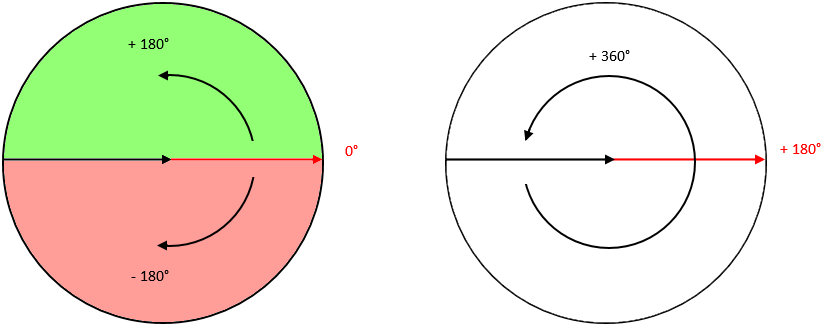
\includegraphics[width=\textwidth]{tree-generation-decision.png}
    \caption{Degree separation method \label{fig:tree-generation-decision}}
\end{figure}

Because a tree can not fully represent a graph, many points exist multiple times in the resulting tree. During recreation of a graph this should be considered.

\FloatBarrier
\pagebreak
\section{K-Means}
Clustering is an approach to group input data. These groups are called clusters. To separate a street network in CPlan into reasonable parts this approach could be used. As described in section \ref{sec:K-Means}, the K-Means algorithm assigns data points to different clusters by using the minimal distances to centroids. For this thesis the position feature (x and y coordinates of the road junctions) are used.

The used feature does ignore the edge data. As a result a cluster is not always connected. This means it could lead to unexpected transitions between clusters.

\subsection{Connected Cluster Approach} \label{sec:connected_cluster_approach}
To solve the problem of unexpected transitions between clusters the best result of the K-Means algorithm tries can be combined with the distance measurement of a \acrlong{APSP} (\acrshort{APSP}) algorithm (Dijkstra / Floyd-Warshall) to assign the edges to a cluster. These algorithms are described in more details in the background chapter \ref{sec:shortest_path}.

\subsection{Additional Features}
Different measurement methods were implemented to rate a created cluster \ref{sec:cluster_analysis_impl}. These features described in section \ref{sec:clusterRating} like the block size or the median street length could be used to cluster the street networks.

\pagebreak
\section{Hierarchical Clustering}
%TODO Short version what singe linkage & PGMA does

\subsection{Hight Memory Usage}
Because WPGMA / UPGMA needs to store all data the memory footprint would be very high. %TODO Describe why exacter.

\subsection{Output Modification}
Idea of output modification
%TODO Describe Idea of output modification!

\pagebreak
\section{Cluster Analysis}
\label{sec:concept_cluster_analysis}
To measure and compare the different areas they should be characterized. Therefore some districts with noticeable characteristics haven been selected an compared to each other. The found characteristics could help to separate a given city on a feature based approach.
These areas have been selected with the aide of Jun.-Prof Dr Reinhard König from the ETH Zurich.

\subsection{Historic District}
\label{sec:historyDistinct}
This district is characterised by a hight count of short streets with many connections. As a result the block areas are small and the block count per area is high. Additionally the mean angles are hight and the density (convex hull area divided by total street length) is low. This characteristics can be observed in the image \ref{fig:historic_district}.

\begin{figure}[!ht]
    \centering
    \begin{mdframed}[style=mdthight, userdefinedwidth=0.4\textwidth, align=center]
        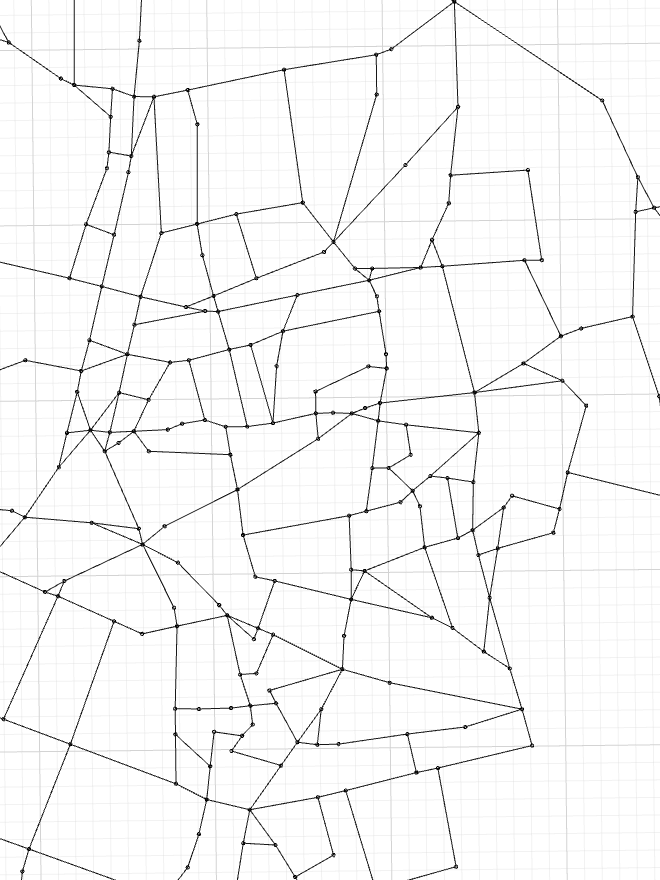
\includegraphics[width=\linewidth]{district_historic.png}
    \end{mdframed}
    \caption{Historic District of Weimar}
    \label{fig:historic_district}
\end{figure}

\FloatBarrier
\subsection{Business/Manhattan District} 
\label{sec:businessDistinct}
If the relative block area (block area divided by surrounding circle area) is high the given subgraph is probably a business/Manhattan district. The mean connection count and the density compared with a historic district \ref{sec:historyDistinct} should be much higher. An example business district can be found on the map of Weimar \ref{fig:business_district}.

\begin{figure}[!ht]
    \centering
    \begin{mdframed}[style=mdthight, userdefinedwidth=0.4\textwidth, align=center]
        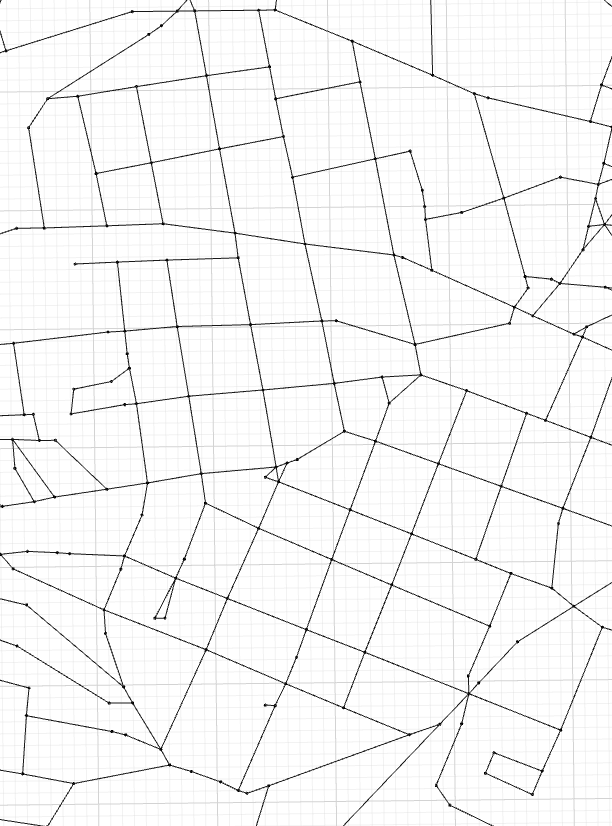
\includegraphics[width=\linewidth]{district_business.png}
    \end{mdframed}
    \caption{Business District of Weimar}
    \label{fig:business_district}
\end{figure}

\FloatBarrier
\subsection{Outskirts Area}
\label{sec:outskits}
These areas are characterized by extreme long streets and a low connection count. As a result the density is very high. The block count is compared with a business or historic district exceptional low. In the image \ref{fig:outskirts_district} these characteristics can be found.

\begin{figure}[!ht]
    \centering
    \begin{mdframed}[style=mdthight, userdefinedwidth=0.6\textwidth, align=center]
        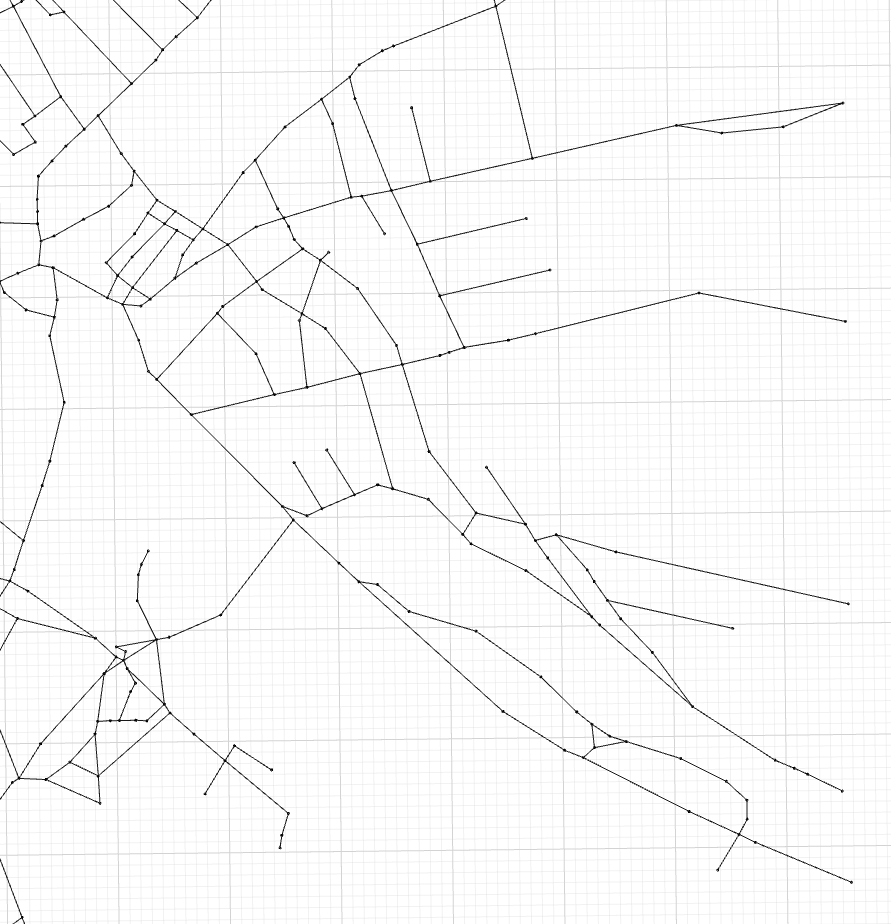
\includegraphics[width=\linewidth]{district_outskirts.png}
    \end{mdframed}
    \caption{Outskirts Area of Weimar}
    \label{fig:outskirts_district}
\end{figure}